\documentclass[12pt,a4paper]{report}
\usepackage{Settings}

%Add Bibliography
\addbibresource{Bibliography.bib}


\begin{document}

% Make title
\begin{titlepage}
    % ETH logo and QuDev
    \noindent
    \begin{minipage}{0.4\textwidth}
        \begin{flushleft}
            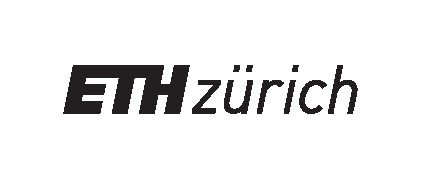
\includegraphics[height=2.0cm]{Title/eth_logo.eps}
        \end{flushleft}
    \end{minipage}
    \hfill
    \begin{minipage}{0.4\textwidth}
        \begin{flushright}
            
\includegraphics[height=1.3cm]{Title/Qudev_logo.pdf} % CHECK: it is not vector!!!
        \end{flushright}
    \end{minipage}

    \vspace{3cm}

    % Title and semester project
    \begin{center}
        \begin{spacing}{2.0}
            {\huge \bfseries Mitigating Crosstalk and Generating Photonic Tree Graph States in Superconducting Circuits}
        \end{spacing}

        \large
        Research Project {\MakeUppercase{\romannumeral 2}}
    \end{center}

    \vspace{1.2cm}

    % Name and email
    \begin{center}
        \large
        Alessandro Azzani

        \begingroup
            \hypersetup{urlcolor=black}
            \href{mailto:aazzani@student.ethz.ch}
            {\texttt{\small aazzani@student.ethz.ch}} 
        \endgroup
    \end{center}

    \vfill

    \begin{center}
        \textbf{Supervisors:} \\
        Alonso Hernández-Antón \\
        Aleksandr Grigorev \\
        Dr. Xi Dai \\

        \vspace{0.3cm}
        \textbf{Principal Investigator:} \\
        Prof. Dr. Andreas Wallraff
    \end{center}

    \vspace{0.5cm}

    % Date
    \begin{center}
        \today
    \end{center}
\end{titlepage}

%Abstract
%Abstract
\thispagestyle{plain}
\newgeometry{left=4.5cm,right=4.5cm}
\pagenumbering{gobble}
\vspace*{3cm}
\begin{center}
    \textbf{\LARGE Abstract}

    \rule{5cm}{0.4pt}

    \vspace{1cm}
\end{center}
% Write your abstract
This study investigates two aspects of quantum information processing with superconducting circuits: microwave signal crosstalk cancellation and the generation of tree graph states. 
Microwave signal crosstalk poses a significant challenge to the fidelity of operations in superconducting qubits for quantum information processing.
We demonstrate the feasibility of cancelling crosstalk using various techniques and pulse shapes.

We also explore the generation of tree graph states, a specific type of many-body entangled state with applications such as one-way quantum repeaters.
These states offer resilience to photon loss, making them useful for robust quantum communication.
We develop a methodology to generate tree graph states using one of our existing device architectures.

\restoregeometry
\newpage

%Start counting in roman numbers
\pagenumbering{roman}

%Table of content
\begingroup
    \hypersetup{linkcolor=black}
    \pagenumbering{gobble}
    \renewcommand\contentsname{\bfseries Contents}
    \tableofcontents
\endgroup


\chapter*{Introduction}
\markboth{INTRODUCTION}{}
\addcontentsline{toc}{chapter}{Introduction}
\label{chap:intro}

Here you write the introduction
%Start counting in arabic numbers
\pagenumbering{arabic}
\chapter{Experimental Setup}
\label{Chap:experimental}

In this chapter we introduce the experimental setup used for our experiments.
We start by presenting the design of our implementation of a qubit: the Transmon.
Then we will show how the qubit is driven for our purposes, in particular how to perform readout and 2-qubit gates.

Finally we put everything together and present the chip used for quantum entangling and photon emission.

\section{The Qubit}
\label{sec:qubit}

The basic idea behind the implementation of a quantum device for quantum information is realizing a 2-level quantum system.
In the Quantum Device Lab this is done through superconducting circuits.
The qubits are star-shaped transmon qubits \cite{transmon_qubits}.
They are characterized by a large capacitor and a SQUID (see \cref{fig:transmon_circuit}).
The latter is flux-tunable and it is made out of two Josephson junctions in parallel.
\begin{figure}[htbp]
    \begin{minipage}[b]{0.5\linewidth}
      \centering
      


\tikzset{every picture/.style={line width=0.75pt}} %set default line width to 0.75pt        

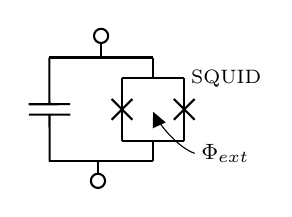
\begin{tikzpicture}[x=0.75pt,y=0.75pt,yscale=-1,xscale=1]
%uncomment if require: \path (0,97); %set diagram left start at 0, and has height of 97

%Shape: Capacitor [id:dp34366919102472526] 
\draw  [line width=0.75]  (20,23.83) -- (20.05,46.33) (30.07,51.31) -- (10.07,51.36) (30.05,46.31) -- (10.05,46.36) (20.07,51.33) -- (20.12,73.83) ;
%Straight Lines [id:da9532858123226031] 
\draw [line width=0.75]    (55,33.83) -- (85,33.83) ;
%Straight Lines [id:da4790035249190253] 
\draw [line width=0.75]    (85,33.83) -- (85,63.83) ;
%Straight Lines [id:da5192559786668693] 
\draw [line width=0.75]    (55,33.83) -- (55,63.83) ;
%Straight Lines [id:da23389027703175358] 
\draw [line width=0.75]    (55,63.83) -- (85,63.83) ;
%Straight Lines [id:da6028752523424945] 
\draw [line width=0.75]    (50,43.83) -- (60,53.83) ;
%Straight Lines [id:da22268293223346158] 
\draw [line width=0.75]    (50,53.83) -- (60,43.83) ;
%Straight Lines [id:da7666685944565205] 
\draw [line width=0.75]    (80,53.83) -- (90,43.83) ;
%Straight Lines [id:da0860971350076063] 
\draw [line width=0.75]    (80,43.83) -- (90,53.83) ;
%Straight Lines [id:da32147396047949894] 
\draw [line width=0.75]    (20,23.83) -- (70,23.83) ;
%Straight Lines [id:da3842851758264739] 
\draw [line width=0.75]    (20,73.83) -- (70,73.83) ;
%Straight Lines [id:da04257544936461244] 
\draw [line width=0.75]    (70,23.83) -- (70,33.83) ;
%Straight Lines [id:da22754146049716317] 
\draw [line width=0.75]    (70,63.83) -- (70,73.83) ;
%Straight Lines [id:da6459112049306985] 
\draw [line width=0.75]    (43.42,79.83) -- (43.42,73.83) ;
%Shape: Circle [id:dp6531205659740902] 
\draw  [line width=0.75]  (40,83.25) .. controls (40,81.36) and (41.53,79.83) .. (43.42,79.83) .. controls (45.3,79.83) and (46.83,81.36) .. (46.83,83.25) .. controls (46.83,85.14) and (45.3,86.67) .. (43.42,86.67) .. controls (41.53,86.67) and (40,85.14) .. (40,83.25) -- cycle ;
%Straight Lines [id:da42435820900303667] 
\draw [line width=0.75]    (45,16.83) -- (45,23.83) ;
%Shape: Circle [id:dp32456243319283773] 
\draw  [line width=0.75]  (48.33,13.33) .. controls (48.38,15.22) and (46.89,16.78) .. (45,16.83) .. controls (43.11,16.88) and (41.55,15.39) .. (41.5,13.5) .. controls (41.45,11.62) and (42.94,10.05) .. (44.83,10) .. controls (46.71,9.95) and (48.28,11.44) .. (48.33,13.33) -- cycle ;

%Curve Lines [id:da7487363329577509] 
\draw [color={rgb, 255:red, 0; green, 0; blue, 0 }  ,draw opacity=1 ]   (90,70) .. controls (83.25,67.65) and (75.22,59.11) .. (71.34,52.55) ;
\draw [shift={(70,50)}, rotate = 65.77] [fill={rgb, 255:red, 0; green, 0; blue, 0 }  ,fill opacity=1 ][line width=0.08]  [draw opacity=0] (7.14,-3.43) -- (0,0) -- (7.14,3.43) -- cycle    ;

% Text Node
\draw (87,33.83) node [anchor=west] [inner sep=0.75pt]   [align=left] {{\scriptsize SQUID}};
% Text Node
\draw (92,70) node [anchor=west] [inner sep=0.75pt]  [font=\footnotesize,color={rgb, 255:red, 0; green, 0; blue, 0 }  ,opacity=1 ] [align=left] {$\displaystyle \Phi _{\text{ext}}$};


\end{tikzpicture}
      \captionsetup{skip=-20pt}
      \caption{Circuit diagram of a transmon qubit}
      \label{fig:transmon_circuit}
    \end{minipage}
    \hfill
    \begin{minipage}[b]{0.45\linewidth}
      \centering
      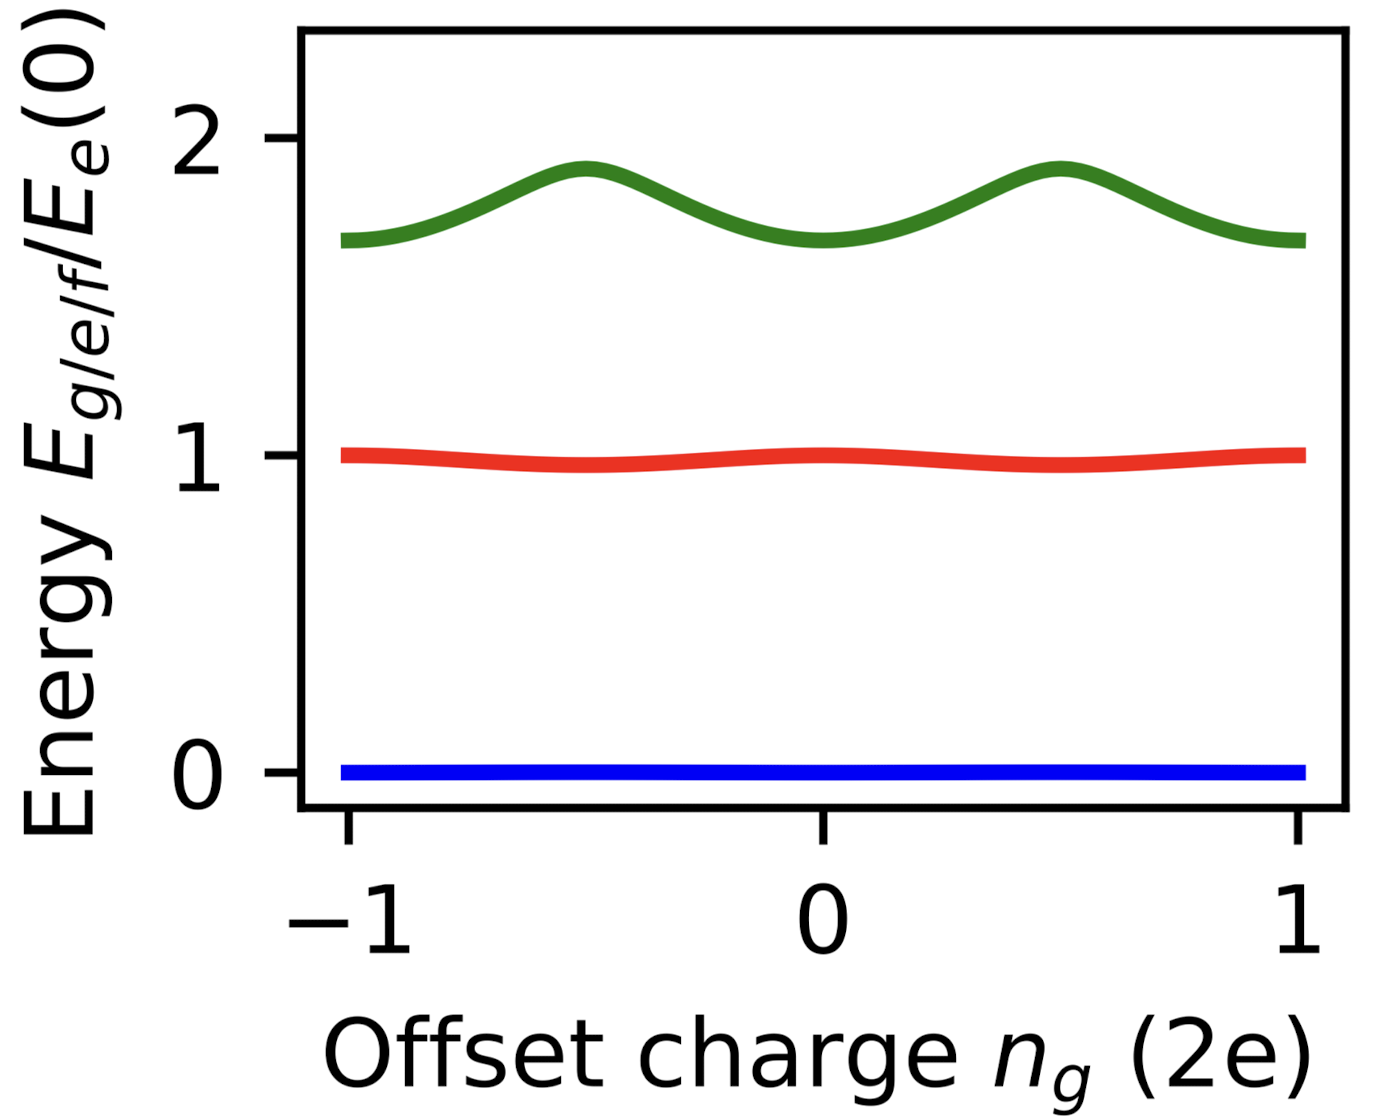
\includegraphics[width = 0.5 \textwidth]{Images/Chap1/Qubit_energy.png}
      \caption{Energy spectrum relative to $N_g$}
      \label{fig:qubit_energy}
    \end{minipage}
  \end{figure}
  

The Hamiltonian representing the dynamics of such a transmon is 
\begin{equation}
    \hat{H} = E_C (\hat{N} - N_g)^2 - E_{J_0, \text{max}} \cos(\pi\frac{\Phi_{\text{ext}}}{\Phi_0})\cos\hat{\delta}
\end{equation}
where $\hat{N}$ is the operator of number of Cooper pairs in the island and $\hat{\delta}$ is the phase operator of the transmon.
This can be seen as a non-linear harmonic oscillator.

By changing the external magnetic flux through the SQUID $\Phi_\text{ext}$, it's possible to change the energy splitting between the first two energy levels $\ket{g}$ and $\ket{e}$, and thus the frequency of the qubit.
Furthermore, the anharmonicity allows us to access the first and second transition separately, since they have different energy gaps (see \cref{fig:qubit_energy}).
Nevertheless, it is important to mention that in our particular setup the qubits are not flux-tunable, because it is not useful for out purposes.
We will present our setup in more detail in \Cref{sec:our_setup}.
\begin{figure}[t]
    \centering
    \begin{subfigure}[b]{0.45\linewidth}
      \centering
      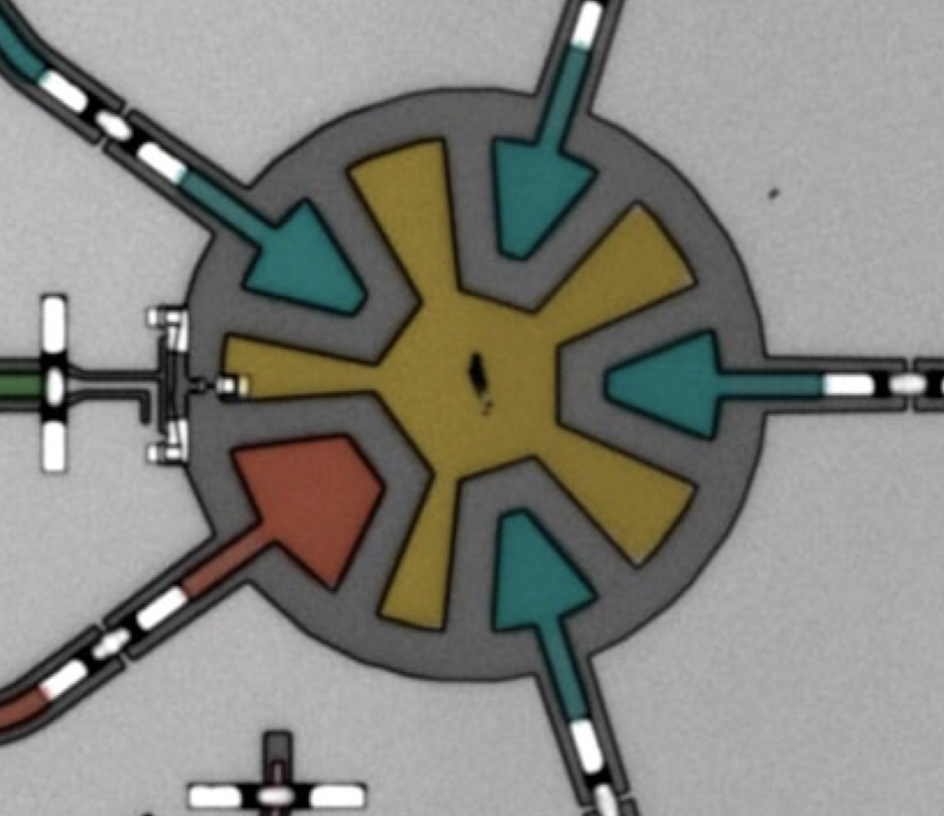
\includegraphics[height=3cm]{Images/Chap1/star_transmon.png}
      \caption{Star-shaped transmon}
      \label{fig:stqr_transmon}
    \end{subfigure}
    \hfill
    \begin{subfigure}[b]{0.45\linewidth}
      \centering
      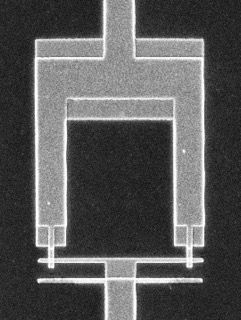
\includegraphics[height=3cm]{Images/Chap1/SQUID.jpeg}
      \caption{Zoom-in of a SQUID loop}
      \label{fig:squid_loop}
    \end{subfigure}
    \caption{Images of the devices used in the lab}
    \label{fig:transmon_squid_images}
  \end{figure}

The qubits are star-shaped and made out of niobium(see \cref{fig:transmon_squid_images}), fabricated on a silicon substrate.

\section{Dispersive Readout}
\label{sec:readout}

The readout mechanism allows us to measure the state of the qubit in a non-demolishing way \cite{singleshot_readout}.
In our experiments this is needed in order to characterize the device and for calibration purposes.

The transmon our capacitively coupled to a readout resonator, which is a waveguide on our device.
By sending through this waveguide a signal far detuned from the qubit's frequency, its frequency will slightly change depending on the state of the qubit, without interfering with the state of the latter.
This process ids described by the James-Cummins Hamiltonian
\begin{equation}
    \hat{H} = \hbar \omega_r \hat{a}^\dagger \hat{a} + \frac{1}{2} \hbar \omega_{ge} \hat{\sigma}^z + \hbar g (\hat{a}^\dagger \hat{\sigma}^- + \hat{a} \hat{\sigma}^+) ,
\end{equation}
which models the coupling between a 2-level system and a light mode in a cavity.
Thus, by measuring the frequency shift of the readout resonator, we are able to infer the qubit's state.

In order to not let the qubit couple too strongly to the environment through the readout resonator, a Purcell filter is applied between the resonator and the qubit.
This allows to keep the lifetimes fo the qubits long, by suppressing spontaneous emission due to the Purcell effect \cite{Purcell_effect}.

\section{Tunable Couplers}
\section{Our Chip}
\label{sec:our_setup}

\chapter{Protocols for 2 qubit gates}
\section{Storage-Storage}
\section{Storage-Emitter}
\subsection{SWAP}
\subsection{CNOT}

%Print bibliography
\printbibliography[heading=bibintoc]

\end{document}